\documentclass[border=2mm]{standalone}
\usepackage{physics}
\usepackage{tikz}
\usepackage{pgfplots}
\pgfplotsset{compat=1.16}

\begin{document}
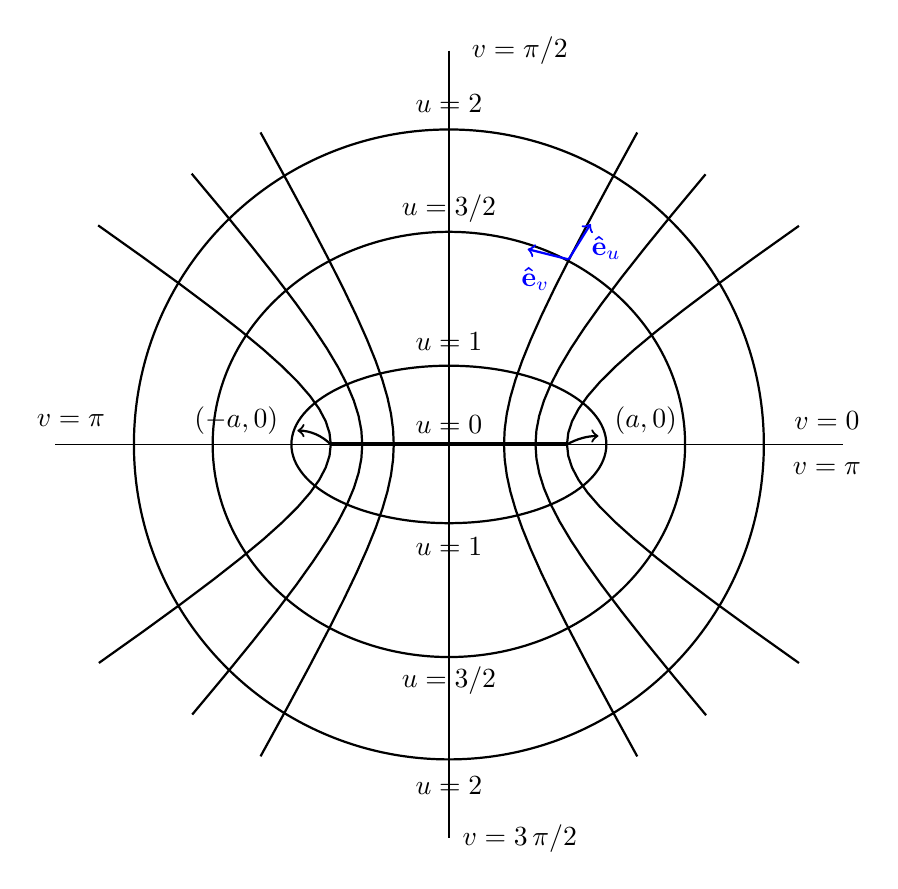
\begin{tikzpicture}[thick]
    \draw [line width=0.2mm] (-5, 0) -- (5, 0);
    \draw [line width=0.2mm] (0, 5) -- (0, -5);
    \draw (0, 0) ellipse (2cm and 1 cm);
    \draw (0, 0) ellipse (3cm and 2.7 cm);
    \draw (0, 0) ellipse (4cm and 4 cm);
    % \node at (-1.5, 0.9) {$u_{1}$};
    % \node at (-2.25, 1.7) {$u_{2}$};

    {
    \pgfmathsetmacro{\a}{1.5}
    \pgfmathsetmacro{\b}{(\a*sqrt((1.2)^2-1)} 
    \draw plot[domain=-1.75:1.75] ({\a*cosh(\x)},{\b*sinh(\x)});
    }
    
    {
    \pgfmathsetmacro{\a}{1.1}
    \pgfmathsetmacro{\b}{(\a*sqrt((1.5)^2-1)} 
    \draw plot[domain=-1.752:1.75] ({\a*cosh(\x)},{\b*sinh(\x)});
    }
    
    {
    \pgfmathsetmacro{\a}{0.7}
    \pgfmathsetmacro{\b}{(\a*sqrt((2)^2-1)} 
    \draw plot[domain=-1.9:1.9] ({\a*cosh(\x)},{\b*sinh(\x)});
    }
    
    {
    \pgfmathsetmacro{\a}{-1.5}
    \pgfmathsetmacro{\b}{(\a*sqrt((1.2)^2-1)} 
    \draw plot[domain=-1.752:1.75] ({\a*cosh(\x)},{\b*sinh(\x)});
    }
    
    {
    \pgfmathsetmacro{\a}{-1.1}
    \pgfmathsetmacro{\b}{(\a*sqrt((1.5)^2-1)} 
    \draw plot[domain=-1.752:1.75] ({\a*cosh(\x)},{\b*sinh(\x)});
    }

    {
    \pgfmathsetmacro{\a}{-0.7}
    \pgfmathsetmacro{\b}{(\a*sqrt((2)^2-1)} 
    \draw plot[domain=-1.9:1.9] ({\a*cosh(\x)},{\b*sinh(\x)});
    }

    \draw[line width=0.5mm] (-1.5, 0) -- (1.5, 0) node [midway, above] {$u = 0$};
    \node at (0, 1.3) {$u = 1$};
    \node at (0, 3) {$u = 3/2$};
    \node at (0, 4.33) {$u = 2$};
    \node at (0, -1.3) {$u = 1$};
    \node at (0, -3) {$u = 3/2$};
    \node at (0, -4.33) {$u = 2$};

    \node at (4.8, 0.3) {$v = 0$};
    \node at (0.9, 5) {$v=\pi/2$};
    \node at (-4.8, 0.3) {$v = \pi$};
    \node at (0.9, -5) {$v= 3 \, \pi/2$};
    \node at (4.8, -0.3) {$v =\pi$};

    \draw [->, color=blue] (1.52, 2.35) -- (1.8, 2.8);
    \draw [->, color=blue] (1.52, 2.35) -- (1, 2.48);

    \node [text= blue] at (2, 2.5) {$\vu{e}_{u}$};
    \node [text= blue] at (1.1, 2.1) {$\vu{e}_{v}$};

    \draw [->] (1.5, 0) arc (120:90:0.8);
    \node at (2.5, 0.3) {$(a, 0)$};
    
    \draw [->] (-1.5, 0) arc (45:90:0.6);
    \node at (-2.7, 0.3) {$(-a, 0)$};

\end{tikzpicture}
\end{document}